\documentclass[runningheads,a4paper]{llncs}

\usepackage[utf8]{inputenc}
\usepackage[T1]{fontenc}
%\usepackage[ngerman]{babel}
\usepackage{enumerate}
\usepackage{marvosym}
\usepackage{gensymb}
\usepackage[bookmarks,bookmarksopen,bookmarksdepth=2]{hyperref}
\usepackage{amsmath}
\usepackage{amsfonts}
\usepackage{amssymb}
%\usepackage{amsthm}
\usepackage{mathrsfs}
\usepackage{fancyhdr}

\usepackage{graphicx}
\graphicspath{{./img/}}

\usepackage[acronym,toc]{glossaries}
\makeglossaries

%\newtheorem{definition}{Definition}
%\newtheorem{theorem}{Theorem}
\newtheorem{axiom}{Axiom}


\newcommand{\partOf}{\text{~partOf~}}
\newcommand{\correspondsTo}{\text{~correspondsTo~}}
\newcommand{\conformsTo}{\text{~conformsTo~}}


\newcommand{\megal}{\textsf{MegaL}~}
\newcommand{\megalxtext}{\textsf{MegaL/Xtext}~}
\newcommand{\megaltext}{\textsf{MegaL/Text}~}
\newcommand{\eclipse}{\textsf{eclipse}~}
\newcommand{\theTitle}{Traceability Recovery \& Exploration in an O/R/X-Mapping scenario with \megal along the mereotopological aspects of software artifacts}

%opening
\title{Exposé for B.Sc. Thesis}

\subtitle{\theTitle}

\author{Maximilian Meffert\\210101205}
\institute{University of Koblenz-Landau}



\begin{document}


\maketitle
%
%\begin{abstract}
%asdf 
%\end{abstract}


\section{Introduction}
This exposé\footnote{\url{http://www.softlang.org/info:expose}} outlines the thesis:
\begin{center}
\it
\theTitle
\end{center}
for acquiring the degree Bachelor Science (B.Sc.) in Computer Science.

The central topic of the thesis will be the study of \megal's traceability capabilities.


\subsubsection{Road-map}
Section \ref{section:Motivation} motivates the topic of the thesis.
\ref{section:ResearchHypthesisAndQuestions} defines a preliminary hypothesis and formulates the research questions.
\ref{section:Objectives} specifies the important objectives for the thesis.
\ref{section:Background} gives a short overview over the necessary background information.
\ref{section:Methodology} describes the approach and methodology of the thesis.
Eventually \ref{section:StructureOfTheThesis} outlines the interim structure of the thesis.


\section{Motivation}
\label{section:Motivation}
A common task for during the development of software systems is to persist and serialize a domain model.
Consider a simple web-service where data is stored in a database and served via HTTP in serialized form, e.g. XML or JSON.



\section{Research Hypotheses \& Questions}
\label{section:ResearchHypthesisAndQuestions}
Research Hypotheses are:
\begin{itemize}
\item[RH1]
If two artifacts are in a Correspondence-Relationship, they contain constituent parts in the same relation to each other, i.e.:
\begin{align*}
&A_1 \correspondsTo A_2
\\&\Rightarrow
\exists a_1, a_2: 
a_1 \partOf A_1 
\wedge a_2 \partOf A_2 
\wedge a_1 \correspondsTo a_2
\end{align*}

\item[RH2]
If two artifacts are in a Conformance-Relationship, they contain constituent parts in the same relation to each other, i.e.:
\begin{align*}
&A_1 \conformsTo A_2
\\&\Rightarrow
\exists a_1, a_2: 
a_1 \partOf A_1 
\wedge a_2 \partOf A_2 
\wedge a_1 \conformsTo a_2
\end{align*}
\end{itemize}

Research Questions are:
\begin{itemize}
\item[RQ1] description
%\item[RQ2] description
%\item[RQ3] description
\end{itemize}

\section{Objectives}
\label{section:Objectives}
Objectives for the thesis are:
\begin{itemize}
\item[O1]
Implementation of a \megalxtext-extension capable of recovering traceability links representing PartOf-, Correspondence- and Conformance-Relationships between code fragments.
\item[O2]
Implementation of a \megalxtext-extension allowing for an user to visually explore traceability links, i.e. PartOf-, Correspondence- and Conformance-Relationships between code fragments.
\item[O3]
Providing an extensive discussion comparing \megal with related approaches on traceability recovery.
\item[O4]
Providing an extensive discussion comparing \megal with related approaches on ontologies for software artifacts or software engineering in general.
%\item[O5] description
%\item[O6] description
\end{itemize}

\section{Background}
\label{section:Background}

\subsection{\megal}
\megal is a Domain Specific Language (DSL) and technology designed  for modeling the linguistic architecture of software systems.
It is actively developed by the Software Language Team\footnote{\url{http://www.softlang.org/}} at the University of Koblenz-Landau and currently has two implementations: 
\begin{itemize}
\item
\megalxtext an \eclipse based Integrated Development Environment (IDE)
\item
and \megaltext a text-file and console based implementation with an 
\end{itemize}
\subsection{Ontologies}
\subsection{Traceability}
\subsection{Mereology}
\subsection{Static \& Dynamic Code Analysis}
\subsection{XML-Binding (JAXB)}
\subsection{Object-Relational-Mapping (JPA/Hibernate)}

\section{Methodology}
\label{section:Methodology}


\begin{figure}
\label{figure:TheCompanyModel}
\centering
\includegraphics[width=.6\textwidth]{companies.png}
\caption{The Company Model}
\end{figure}

\begin{figure}
\label{figure:TheCompanyInstanceCalledSoftlangInc}
\centering
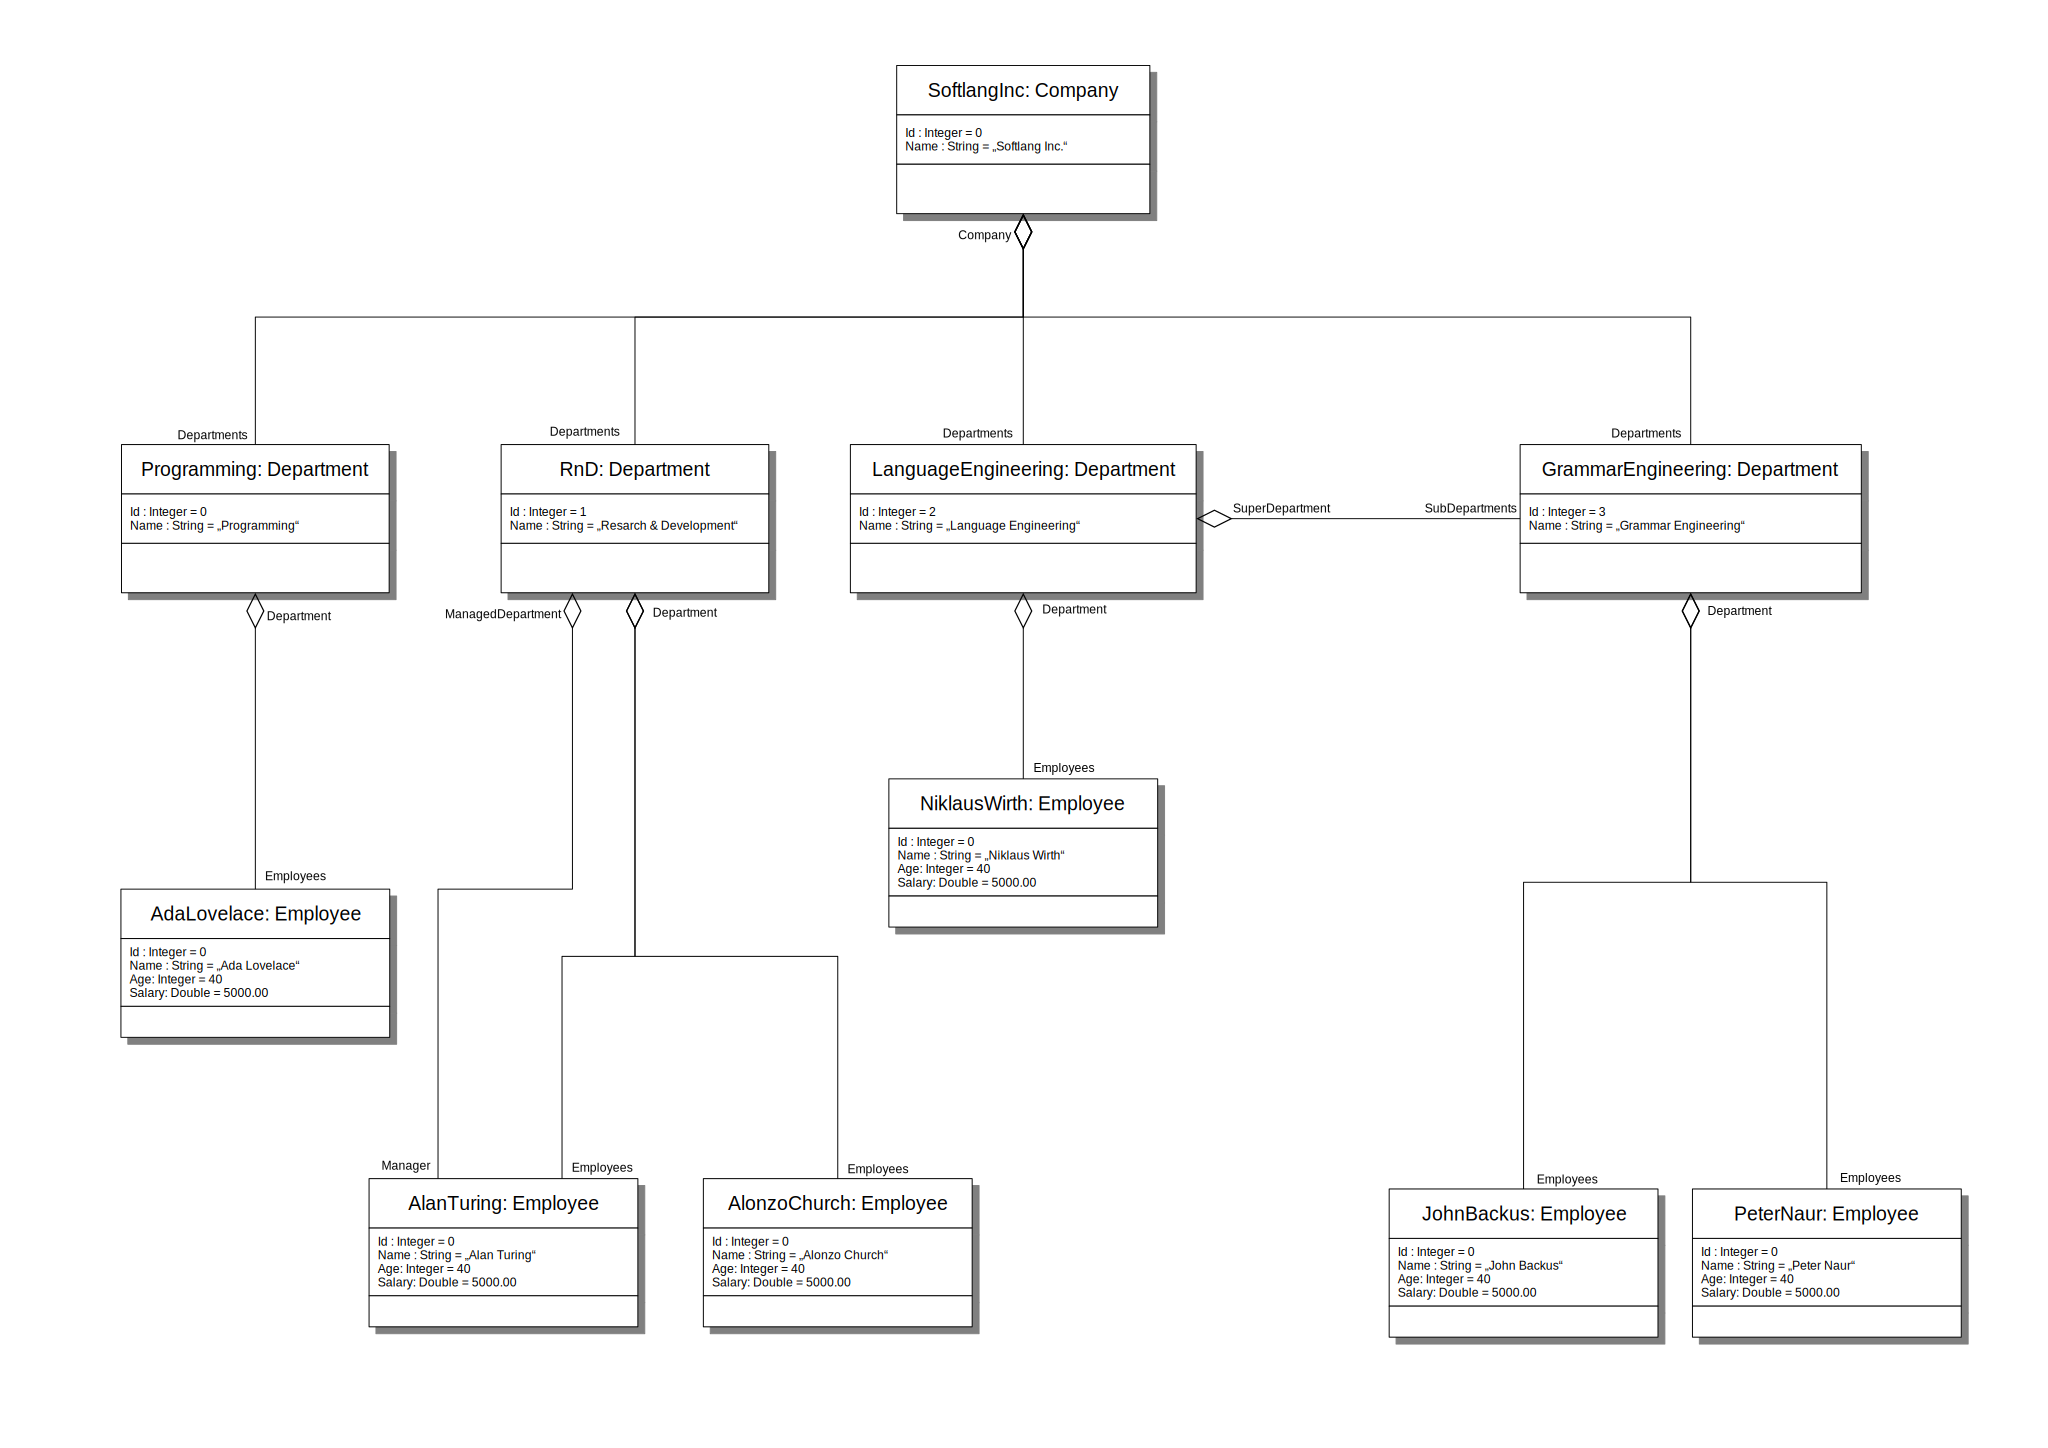
\includegraphics[width=.9\textwidth]{softlanginc.png}
\caption{The Company Instance called \textit{Softlang Inc.}}
\end{figure}

\section{Structure of the Thesis}
\label{section:StructureOfTheThesis}

\begin{figure}
\begin{center}
\begin{minipage}[t]{0.5\textwidth}
\begin{enumerate}

\item
\textbf{Introduction}

\item
\textbf{Background}

\item
\textbf{Related Work}

\item
\textbf{Methodology}

\item
\textbf{Requirements}

\item
\textbf{Design}

\item
\textbf{Implementation}

\item
\textbf{Case Study}

\item
\textbf{Analysis/Results}

\item
\textbf{Conclusion}

\end{enumerate}
\end{minipage}
\end{center}
\caption{Structure of the Thesis}
\end{figure}



\url{http://softlang.wikidot.com/info:thesis-structure}

\cite{DBLP:conf/ecmdafa/LammelV14}
\cite{DBLP:conf/models/FavreLV12}
\cite{DBLP:journals/dke/Varzi96}
\cite{DBLP:journals/entcs/FavreN05}
\cite{Softlang:course/ptt15/technoloymodeling}
\cite{DBLP:conf/sle/Lammel16}

\bibliographystyle{splncs}
\bibliography{../bsc}{}

%\printglossaries
%\printglossary[type=\acronymtype]

\end{document}
